\documentclass[12pt]{article}
\usepackage{parskip}
\usepackage[letterpaper, margin=1in]{geometry}
\usepackage{listings}
\usepackage{verbatim}
\usepackage{tikz}
\usepackage{subcaption}
\usepackage{amsmath}
\usepackage{graphicx}
\usepackage{multirow}
\graphicspath{{./images/}}
\usetikzlibrary{matrix}

\title{COMPENG 2SI4 LAB 1 \& 2 REPORT}
\author{Raeed Hassan \\ hassam41 \\  \\ McMaster University}

\newcommand{\code}[1]{\texttt{#1}}

\begin{document}
\maketitle
\pagebreak

\section*{Description of Data Structures and Algorithms}
%Describe the data structure used to implement the HugeIntegerclass and how you implemented each operation (comparison, addition, subtraction, multiplication).In other words, describe how the integer is stored, what additional variables youneed to maintain, etc. Describe in detail the algorithm used to implement each operation. Include figures to illustrate your algorithms (for example, show the data structure before, in the middle and after the execution of each method).
The \code{HugeInteger} class has two private fields, \code{int sign} that stores the sign of the integer as an integer and \code{int[] magnitude} that stores the digits of the integer in an integer array.

The addition operation \code{public HugeInteger add(HugeInteger h)} returns a \code{HugeInteger sum} that represents the integer sum of \code{this} and \code{h}. It first checks if either \code{this} or \code{h} are zero by checking if \code{sign == 0}. The method returns the non-zero \code{HugeInteger} if one \code{HugeInteger} is 0 and returns a \code{HugeInteger} representing 0 if both are 0. Otherwise, the general algorithm is to create a new \code{HugeInteger sum} with size of \code{magnitude} equal to the larger \code{magnitude.length} between \code{this} and \code{h} and iterate through \code{this.magnitude} and \code{h.magnitude} to add the values at every index of the arrays multiplied by their respective \code{sign} to \code{sum.magnitude}. After this process, we iterate through \code{sum.magnitude} in reverse order to fix elements that are greater than 9 or less than 0. If it is greater than 9, subtract 10 from current index and add 1 to the previous index. If it is less than 0, increase the current index by 10 and subtract 1 from the previous index. All leading zeros are removed from \code{sum.magnitude} afterwards by replacing it with a smaller array. If the first index of \code{sum.magnitude} is greater than 9, a new array of length \code{sum.magnitude.length+1} is created and the values of \code{sum.magnitude} are copied over. This new matrix replaces \code{sum.magnitude}. The method then removes all leading zeros from \code{sum.magnitude}. The value of \code{sum.sign} equals the 1 if both integers were positive or if the first element of \code{sum.magnitude} is positive if the signs of the integers did not match. The value of \code{sum.sign} equals -1 if both integers were negative or if the first element of \code{sum.magnitude} is negative if the signs of the integers did not match. The method finally returns \code{HugeInteger sum}. The entire process is illustrated in Figure 1 with two positive integers.
\begin{figure}[h!]
    \def\arrh{3,7,1,9,4,7}
    \def\arrthis{8,4,6,6,4,8}
    \centering
    \begin{subfigure}[b]{0.475\textwidth}
        \centering
        \newcounter{ind}
        \begin{tikzpicture}
        % size of each node   
        \def\sz{8mm}
        % node style definition
        \tikzstyle{block} = [
        draw, rectangle,
        minimum height=\sz, minimum width=\sz ];    
        \tikzstyle{plain} = [draw=none,fill=none];
        % array element definition
        \def\arrsum{0,0,0,0,0,0};
        %\def\black{1,2,3,4,5,7,9,10,11};
        \def\y{0}; % y pos of arr
        \setcounter{ind}{0};
        \node[plain] at (0,\y) { this };
        \foreach \item in \arrthis
        {
            \addtocounter{ind}{1};
            \node[block] at (\theind*\sz,\y+0) { \item };
            %\node[plain] at (\theind*\sz,\y+0.7) { \theind };
        }
        \def\y{-1}; % y pos of arr
        \setcounter{ind}{0};
        %\setcounter{indx}{-1};
        \node[plain] at (0,\y) { h };
        \foreach \item in \arrh
        {
            \addtocounter{ind}{1};
            %\addtocounter{indx}{1};
            \node[block] at (\theind*\sz,\y+0) { \item };
            %\node[plain] at (\theind*\sz,\y+0.7) { \theindx };
        }
        \def\y{-2}; % y pos of arr
        \setcounter{ind}{0};
        %\setcounter{indx}{-2};
        \node[plain] at (0,\y) { sum };
        \foreach \item in \arrsum
        {
            \addtocounter{ind}{1};
            %\addtocounter{indx}{1};
            \node[block] at (\theind*\sz,\y+0) { \item };
            %\node[plain] at (\theind*\sz,\y+0.7) { \theindx };
        }
        \end{tikzpicture}
        \caption{initialize \code{sum}}
    \end{subfigure}
    \hfill
    \begin{subfigure}[b]{0.475\textwidth}
        \centering
        \newcounter{inda}
        \begin{tikzpicture}
        % size of each node   
        \def\sz{8mm}
        % node style definition
        \tikzstyle{block} = [
        draw, rectangle,
        minimum height=\sz, minimum width=\sz ];    
        \tikzstyle{plain} = [draw=none,fill=none];
        % array element definition
        \def\arrsum{8,4,6,6,4,8};
        %\def\black{1,2,3,4,5,7,9,10,11};
        \def\y{0}; % y pos of arr
        \setcounter{inda}{0};
        \node[plain] at (0,\y) { this };
        \foreach \item in \arrthis
        {
            \addtocounter{inda}{1};
            \node[block] at (\theinda*\sz,\y+0) { \item };
        }
        \def\y{-1}; % y pos of arr
        \setcounter{inda}{0};
        \node[plain] at (0,\y) { h };
        \foreach \item in \arrh
        {
            \addtocounter{inda}{1};
            \node[block] at (\theinda*\sz,\y+0) { \item };
        }
        \def\y{-2}; % y pos of arr
        \setcounter{inda}{0};
        \node[plain] at (0,\y) { sum };
        \foreach \item in \arrsum
        {
            \addtocounter{inda}{1};
            \node[block] at (\theinda*\sz,\y+0) { \item };
        }
        \end{tikzpicture}
        \caption{add \code{this} to \code{sum}}
    \end{subfigure}
    \vskip\baselineskip
    \begin{subfigure}[b]{0.475\textwidth}
        \centering
        \newcounter{indb}
        \begin{tikzpicture}
        % size of each node   
        \def\sz{8mm}
        % node style definition
        \tikzstyle{block} = [
        draw, rectangle,
        minimum height=\sz, minimum width=\sz ];    
        \tikzstyle{plain} = [draw=none,fill=none];
        % array element definition
        \def\arrsum{11,11,7,15,8,15};
        \def\y{0}; % y pos of arr
        \setcounter{indb}{0};
        \node[plain] at (0,\y) { this };
        \foreach \item in \arrthis
        {
            \addtocounter{indb}{1};
            \node[block] at (\theindb*\sz,\y+0) { \item };
        }
        \def\y{-1}; % y pos of arr
        \setcounter{indb}{0};
        %\setcounter{indx}{-1};
        \node[plain] at (0,\y) { h };
        \foreach \item in \arrh
        {
            \addtocounter{indb}{1};
            \node[block] at (\theindb*\sz,\y+0) { \item };
        }
        \def\y{-2}; % y pos of arr
        \setcounter{indb}{0};
        %\setcounter{indx}{-2};
        \node[plain] at (0,\y) { sum };
        \foreach \item in \arrsum
        {
            \addtocounter{indb}{1};
            \node[block] at (\theindb*\sz,\y+0) { \item };
        }
        \end{tikzpicture}
        \caption{add \code{h} to \code{sum}}
    \end{subfigure}
    \hfill
    \begin{subfigure}[b]{0.427\textwidth}
        \centering
        \newcounter{indc}
        \begin{tikzpicture}
        % size of each node   
        \def\sz{8mm}
        % node style definition
        \tikzstyle{block} = [
        draw, rectangle,
        minimum height=\sz, minimum width=\sz ];
        \tikzstyle{plain} = [draw=none,fill=none];
        % array element definition
        \def\arrsum{1,2,1,8,5,9,5};
        \def\y{0}; % y pos of arr
        \setcounter{indc}{0};
        \node[plain] at (0,\y) { this };
        \foreach \item in \arrthis
        {
            \addtocounter{indc}{1};
            \node[block] at (\theindc*\sz,\y+0) { \item };
        }
        \def\y{-1}; % y pos of arr
        \setcounter{indc}{0};
        \node[plain] at (0,\y) { h };
        \foreach \item in \arrh
        {
            \addtocounter{indc}{1};
            \node[block] at (\theindc*\sz,\y+0) { \item };
        }
        \def\y{-2}; % y pos of arr
        \setcounter{indc}{0};
        \node[plain] at (0,\y) { sum };
        \foreach \item in \arrsum
        {
            \addtocounter{indc}{1};
            \node[block] at (\theindc*\sz,\y+0) { \item };
        }
        \end{tikzpicture}
        \caption{reduce elements to 1 digit}
    \end{subfigure}
    \caption{Addition}
\end{figure}

The subtraction operation \code{public HugeInteger subtract(HugeInteger h)} returns a \\ \code{HugeInteger difference} that represents the integer given by of \code{h} subtracted from \code{this}. simply creates a \code{HugeInteger temp} with the same \code{magnitude} as \code{HugeInteger h} but the opposite \code{sign} and returns the \code{HugeInteger} that is returned by calling the add method \code{this.add(temp)}.

The multiplication operation returns a \code{HugeInteger product} that represents the integer product of \code{this} and \code{h}. It first checks if either \code{this.sign == 0} or \code{h.sign == 0}, in which case it will return a \code{HugeInteger} representing $0$. Otherwise, the general algorithm is to create a $2n+1$ digit \code{HugeInteger product}, then add the products of \code{this.magnitude} and \code{h.magnitude} to \code{product.magnitude}. The operation loops has a nested for loop that iterates through \code{h.magnitude} in the outer loop, and iterates through \code{this.magnitude} in the inner loop, adding \code{this.magnitude*h.magnitude} to \code{product.magnitude} after each iteration of the inner loop. After each iteration of the outer loop, the starting index for \code{product.magnitude} is shifted to the left. After the completion of the nested for loop, the method reduces every element of \code{this.magnitude} to 1 digit, iterating through the array in reverse order and adding \code{product.magnitude[i]/10} to the previous element and setting \code{product.magnitude[i]} equal to \code{product.magnitude[i]\%10}. The method then removes all leading zeros from \code{product.magnitude}. The value of \code{product.sign} is equal to \code{this.sign*h.sign}. The method finally returns \code{HugeInteger product}. The entire process is illustrated in Figure 2 with two positive integers. 
\begin{figure}[h!]
    \def\arrh{9,9}
    \def\arrthis{9,9}
    \centering
    \begin{subfigure}[b]{0.475\textwidth}
        \centering
        \newcounter{indd}
        \begin{tikzpicture}
        % size of each node   
        \def\sz{8mm}
        % node style definition
        \tikzstyle{block} = [
        draw, rectangle,
        minimum height=\sz, minimum width=\sz ];    
        \tikzstyle{plain} = [draw=none,fill=none];
        % array element definition
        \def\arrsum{0,0,0,0};
        %\def\black{1,2,3,4,5,7,9,10,11};
        \def\y{0}; % y pos of arr
        \setcounter{indd}{0};
        \node[plain] at (0,\y) { this };
        \foreach \item in \arrthis
        {
            \addtocounter{indd}{1};
            \node[block] at (\theindd*\sz,\y+0) { \item };
            %\node[plain] at (\theindd*\sz,\y+0.7) { \theindd };
        }
        \def\y{-1}; % y pos of arr
        \setcounter{indd}{0};
        %\setcounter{indx}{-1};
        \node[plain] at (0,\y) { h };
        \foreach \item in \arrh
        {
            \addtocounter{indd}{1};
            %\addtocounter{indx}{1};
            \node[block] at (\theindd*\sz,\y+0) { \item };
            %\node[plain] at (\theindd*\sz,\y+0.7) { \theindx };
        }
        \def\y{-2}; % y pos of arr
        \setcounter{indd}{0};
        %\setcounter{indx}{-2};
        \node[plain] at (0,\y) { prd };
        \foreach \item in \arrsum
        {
            \addtocounter{indd}{1};
            %\addtocounter{indx}{1};
            \node[block] at (\theindd*\sz,\y+0) { \item };
            %\node[plain] at (\theindd*\sz,\y+0.7) { \theindx };
        }
        \end{tikzpicture}
        \caption{initialize \code{product}}
    \end{subfigure}
    \hfill
    \begin{subfigure}[b]{0.475\textwidth}
        \centering
        \newcounter{inde}
        \begin{tikzpicture}
        % size of each node   
        \def\sz{8mm}
        % node style definition
        \tikzstyle{block} = [
        draw, rectangle,
        minimum height=\sz, minimum width=\sz ];    
        \tikzstyle{plain} = [draw=none,fill=none];
        % array element definition
        \def\arrsum{0,0,81,81};
        %\def\black{1,2,3,4,5,7,9,10,11};
        \def\y{0}; % y pos of arr
        \setcounter{inde}{0};
        \node[plain] at (0,\y) { this };
        \foreach \item in \arrthis
        {
            \addtocounter{inde}{1};
            \node[block] at (\theinde*\sz,\y+0) { \item };
        }
        \def\y{-1}; % y pos of arr
        \setcounter{inde}{0};
        \node[plain] at (0,\y) { h };
        \foreach \item in \arrh
        {
            \addtocounter{inde}{1};
            \node[block] at (\theinde*\sz,\y+0) { \item };
        }
        \def\y{-2}; % y pos of arr
        \setcounter{inde}{0};
        \node[plain] at (0,\y) { prd };
        \foreach \item in \arrsum
        {
            \addtocounter{inde}{1};
            \node[block] at (\theinde*\sz,\y+0) { \item };
        }
        \end{tikzpicture}
        \caption{first iteration of outer loop}
    \end{subfigure}
    \vskip\baselineskip
    \begin{subfigure}[b]{0.475\textwidth}
        \centering
        \newcounter{indf}
        \begin{tikzpicture}
        % size of each node   
        \def\sz{8mm}
        % node style definition
        \tikzstyle{block} = [
        draw, rectangle,
        minimum height=\sz, minimum width=\sz ];    
        \tikzstyle{plain} = [draw=none,fill=none];
        % array element definition
        \def\arrsum{0,81,162,81};
        \def\y{0}; % y pos of arr
        \setcounter{indf}{0};
        \node[plain] at (0,\y) { this };
        \foreach \item in \arrthis
        {
            \addtocounter{indf}{1};
            \node[block] at (\theindf*\sz,\y+0) { \item };
        }
        \def\y{-1}; % y pos of arr
        \setcounter{indf}{0};
        %\setcounter{indx}{-1};
        \node[plain] at (0,\y) { h };
        \foreach \item in \arrh
        {
            \addtocounter{indf}{1};
            \node[block] at (\theindf*\sz,\y+0) { \item };
        }
        \def\y{-2}; % y pos of arr
        \setcounter{indf}{0};
        %\setcounter{indx}{-2};
        \node[plain] at (0,\y) { prd };
        \foreach \item in \arrsum
        {
            \addtocounter{indf}{1};
            \node[block] at (\theindf*\sz,\y+0) { \item };
        }
        \end{tikzpicture}
        \caption{second iteration of outer loop}
    \end{subfigure}
    \hfill
    \begin{subfigure}[b]{0.475\textwidth}
        \centering
        \newcounter{indg}
        \begin{tikzpicture}
        % size of each node   
        \def\sz{8mm}
        % node style definition
        \tikzstyle{block} = [
        draw, rectangle,
        minimum height=\sz, minimum width=\sz ];
        \tikzstyle{plain} = [draw=none,fill=none];
        % array element definition
        \def\arrsum{9,8,0,1};
        \def\y{0}; % y pos of arr
        \setcounter{indg}{0};
        \node[plain] at (0,\y) { this };
        \foreach \item in \arrthis
        {
            \addtocounter{indg}{1};
            \node[block] at (\theindg*\sz,\y+0) { \item };
        }
        \def\y{-1}; % y pos of arr
        \setcounter{indg}{0};
        \node[plain] at (0,\y) { h };
        \foreach \item in \arrh
        {
            \addtocounter{indg}{1};
            \node[block] at (\theindg*\sz,\y+0) { \item };
        }
        \def\y{-2}; % y pos of arr
        \setcounter{indg}{0};
        \node[plain] at (0,\y) { prd };
        \foreach \item in \arrsum
        {
            \addtocounter{indg}{1};
            \node[block] at (\theindg*\sz,\y+0) { \item };
        }
        \end{tikzpicture}
        \caption{reduces elements to 1 digit}
    \end{subfigure}
    \caption{Multiplication}
\end{figure}


The comparison operation \code{public int compareTo(HugeInteger h)} returns 1 if \\ \code{this HugeInteger > h}, 0 if \code{this HugeInteger == h}, and -1 if \code{this HugeInteger < h}. The method first compares the values of \code{this.sign} and \code{h.sign}. If \code{this.sign > h.sign}, the method returns 1 as \code{this HugeInteger} is greater. If \code{this.sign < h.sign}, the method returns -1 as \code{HugeInteger h} is greater. If neither condition is satisfied, both integers must have the same value of \code{sign}. If both integers are positive, it will compare their sizes and return 1 if \code{this.magnitude.length > h.magnitude.length} and -1 if \\ \code{this.magnitude.length < h.magnitude.length}. If their lengths are the same, then it will iterate through both arrays and compare the values at each index, returning 1 if \code{this.magnitude[i] > h.magnitude[i]} at an index or -1 if \code{this.magnitude[i] <} \\ \code{h.magnitude[i]} at an index. If both integers are negative, it will go through the same process, however the value returned will be the negative of what is returned with positive integers in each scenario. If none of these conditions have been meet, then the method will \code{return 0} as the two integers are equal.   

\section*{Theoretical Analysis of Running Time and Memory Requirement}
% You also have to compute the amount of memory (in bytes) required to store aninteger of n decimal digits using your HugeInteger class.  You should be ableto derive a formula for the number of bytes required to store your integer, as afunction of the number of decimal digitsnand plot it in a figure.
% Using big-Theta notation, compute the running time (in the worst case and inthe average case) and the amount of extra memory requirementfor each of theoperations (addition, subtraction, comparison, multiplication). Include a detaileddescription of how you arrived at these results.
The \code{HugeInteger} class has fields \code{int sign} and \code{int[] magnitude}. An integer in \code{Java} is stored using 4 bytes. Therefore, the memory required to store a \code{HugeInteger} is $4+4n$, 4 bytes to store \code{sign} and $4n$ bytes to store \code{magnitude}. A plot of the memory required for a \code{HugeInteger} of n decimal digits can be seen in Figure 3.
\begin{figure}[h!]
    \centering
    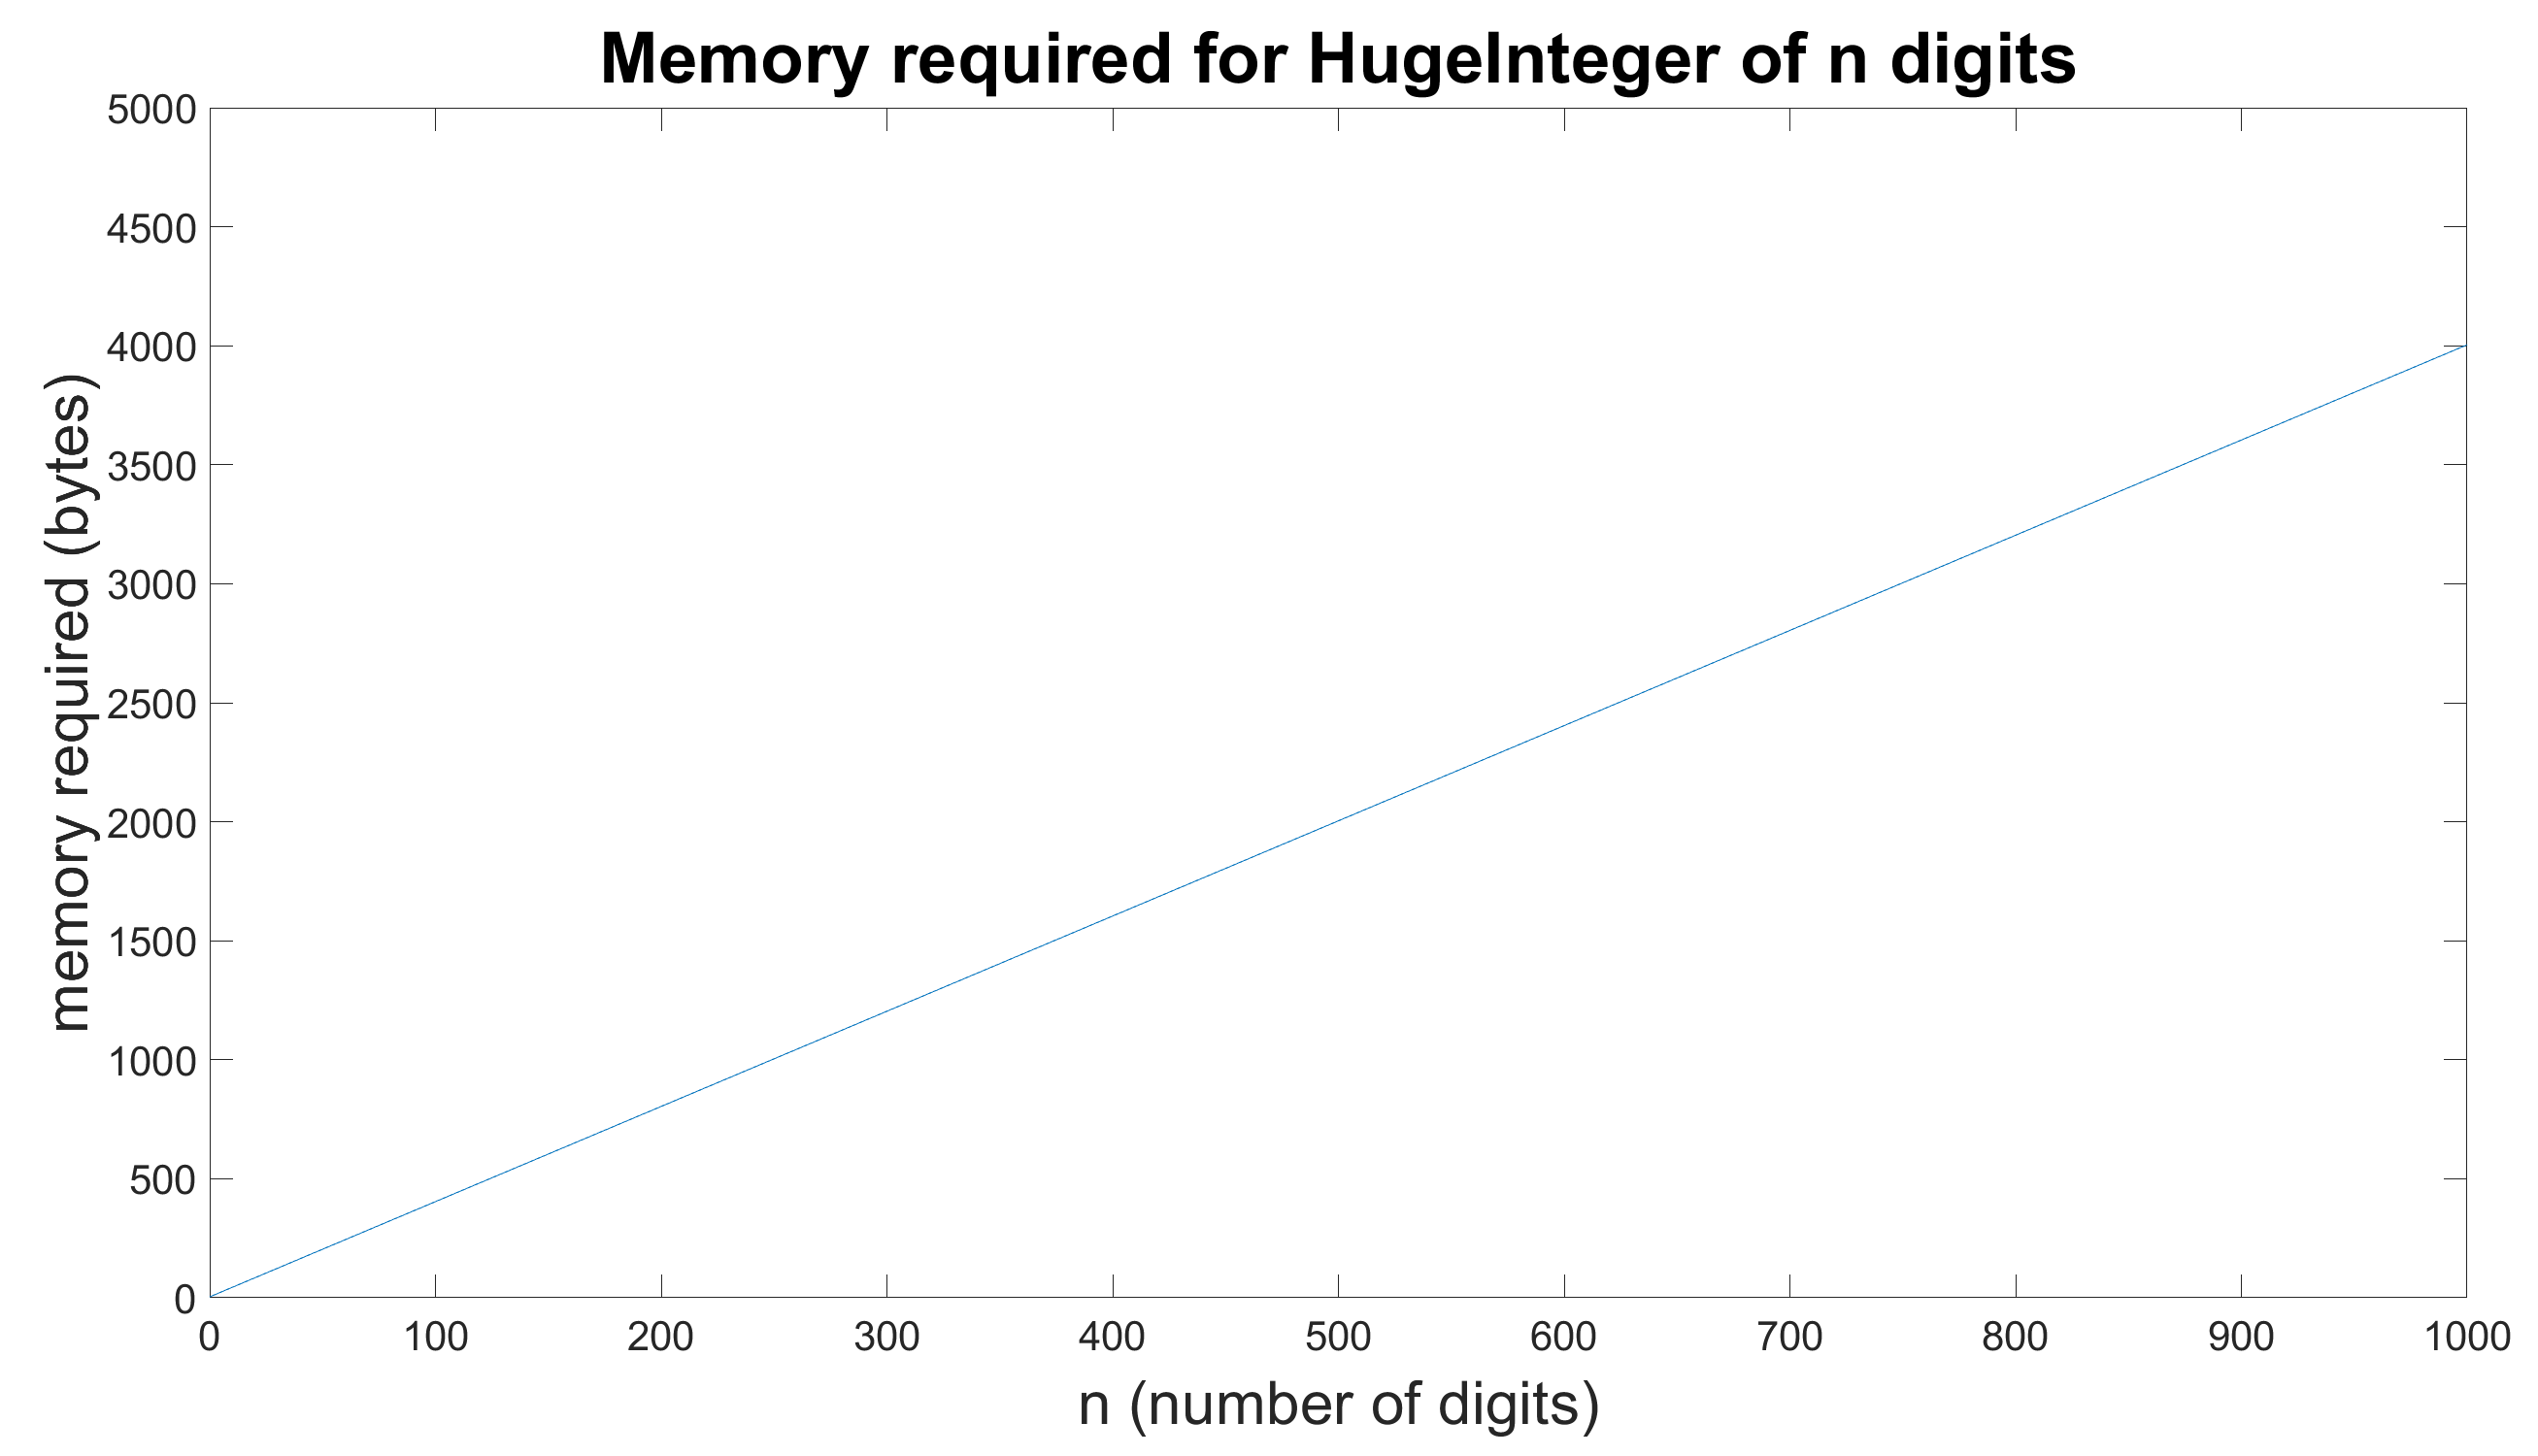
\includegraphics[width=\textwidth]{memoryplot.png}
    \caption{Memory required store a \code{HugeInteger} of $n$ decimal digits}
\end{figure} \\
The running time for the addition operation is $\Theta(n)=n$ for both the average and worst case. The add method consists of operations that take constant time and for loops that take $n$ time. This results in the running time of the operation being $T(n) = c_1n + c_2 = \Theta(n)=n$ in both the average and worst case, as the method will always encounter a for loop. The addition operation requires up to $2(4+4(n+1))$ extra bytes of memory to store the \code{HugeInteger} objects that will be returned, an additional $8n-12n$ bytes of memory to store temporary integer arrays, and up to another $16$ bytes of memory to store several integers. 

The running time for the subtraction operation is $\Theta(n)=n$ for both the average and worst case. The subtract method creates a new \code{HugeInteger temp} to represent the negative of \code{HugeInteger h} and then adds \code{this HugeInteger} and \code{temp}. As the method simply creates a new object (which takes constant time) and then calls add, the running time is $c + T(add) = T(n) = c_1n + c_2 = \Theta(n)=n$ in both the average and worst case, as the method will always encounter a for loop. The subtraction operation requires the additional memory required by the addition operation as it calls the add method and also an additional $4+4n$ bytes to store \code{HugeInteger temp}.

The running time for the multiplication operation is $\Theta(n)=n^2$ for both the average and worst case. The multiplication method consists of operations that take constant time, for loops that take $n$ time, and nested for loops that take $n^2$ time. This results in the running time of the operation being $T(n) = c_1n^2 + c_2n + c_3= \Theta(n)=n^2$ in both the average and worst case, as the method will always encounter a nested for loop. The multiplication operation requires up to $4+4(2n+1)$ extra bytes of memory to store \code{HugeInteger} that will be returned, an additional $8n-12n$ bytes of memory to store temporary integer arrays, and an additional $4$ bytes of memory to store an \code{int} that contains the size of the product.

The running time for the comparison operation is $\Theta(n)=1$ for the average case and $\Theta(n)=n$ for the worst case. The comparison method consists of operations that take constant time and for loops that take $n$ time. This results in the running time of the operation being $T(n) = c_1 = \Theta(n)=1$ in the average case where the method does not encounter a for loop and $T(n) = c_1n + c_2 = \Theta(n)=n$ in the worst case where the method encounters a for loop. The comparison operation requires no additional memory.

\section*{Test Procedure}
% Design a test procedure and justify that it demonstrates thecomplete functionalityof yourHugeIntegerclass.
% What are the possible cases that can arise? What inputs will you use to test thatall the special cases work correctly? What inputs will you use to ensure each ofthe required operations are functioning properly?
% Do your outputs meet the specifications?
% Did you have any difficulties in debugging the code?
% Are there any input conditions that you could not check?
To test the functionality of the \code{HugeInteger} class and its methods, we will create a test class \code{TestHugeInteger} and perform all possible operations on all possible cases. The constructor and all four operations will be tested.

Possible constructor cases including inputs tested: 
\begin{itemize}
    \item input is zero ("0")
    \item input is multiple zeros ("00000")
    \item input is negative zero ("-0")
    \item input is negative with multiple zeros ("-00000")
    \item input is valid string ("1510239")
    \item input is valid string with leading zeros ("000000001510239")
    \item input is valid negative string ("-690290384")
    \item input is negative single digit with leading zeros ("-00000000690290384")
    \item input is invalid positive string input with string in middle ("11234-1231) 
    \item input is invalid negative string input with string in middle ("-1863495-105328403924")
    \item input is $n = 0$ (0)
    \item input is $n > 0$ (5)
    \item input is $n < 0$ (-5)
\end{itemize}
Possible addition cases including inputs tested:
\begin{itemize}
    \item zero + zero ($0 + 0$)
    \item zero + positive ($0 + 123$)
    \item zero + negative ($0 + (-123)$)
    \item two positive integers with different number of digits ($125123 + 173452341$)
    \item two postive integers with same number of digits with same number of digits in result ($212361 + 501293$) 
    \item two postive integers with same number of digits with different number of digits in result ($512315 + 941238$) 
    \item two negative integers with different number of digits ($(-123) + (-6789)$)
    \item two negative integers with same number of digits with same number of digits in result ($(-4424) + (-1138)$) 
    \item two negative integers with same number of digits with different number of digits in result ($(-999) + (-998)$)
    \item positive + negative with positive result ($514 + (-12)$) 
    \item positive + negative with leading zeros in positive result ($999 + (-996)$)
    \item positive + negative with negative result ($913 + (-1042)$) 
    \item positive + negative with leading zeros in negative result ($555 + (-564)$)
\end{itemize}
Possible subtraction cases including inputs tested:
\begin{itemize}
    \item zero - zero ($0 - 0$)
    \item zero - positive ($0 - 123$)
    \item zero - negative ($0 - (-123)$)
    \item positive - zero ($123 - 0$)
    \item negative - zero ($(-123) - 0$)
    \item two positive integers with positive result ($1235 - 123$)
    \item two positive integers with negative result ($125123 - 173452341$)
    \item two positive integers with leading zeros in result ($555 - 564$)
    \item two equal positive integers ($123 - 123$)
    \item two negative integers with positive result ($(-123) - (-1234)$)
    \item two negative integers with negative result ($(-1234) - (-123)$)
    \item two negative integers with leading zeros in result ($(-555) - (-564)$)
    \item two equal negative integers ($(-123) - (-123)$)
    \item positive - negative ($514 - (-123)$) 
    \item negative - positive ($(-514) - 123$)
    \item positive - negative with negative result ($913 + (-1042)$) 
    \item positive - negative with leading zeros in negative result ($555 + (-564)$)
\end{itemize}
Possible multiplication cases including inputs tested:
\begin{itemize}
    \item zero $\times$ zero ($0 \times 0$)
    \item zero $\times$ positive ($0 \times 1$)
    \item zero $\times$ negative ($0 \times -1$)
    \item positive $\times$ positive ($12 \times 99$)
    \item positive $\times$ negative ($12 \times (-99)$)
    \item negative $\times$ negative ($(-12) \times (-99)$)
\end{itemize}
Possible comparison cases including inputs tested:
\begin{itemize}
    \item zero to positive (0, 123)
    \item zero to negative (0, -123)
    \item zero to zero (0, 0)
    \item positive to negative (123,-123)
    \item postive to zero (123,0)
    \item negative to positive (-123, 123)
    \item negative to zero (-123, 0)
    \item positive to larger positive (123, 124)
    \item positive to smaller positive (123, 12)
    \item equal positives (123, 123)
    \item negative to larger negative (-123, -12)
    \item negative to smaller negative (-123, -124)
    \item equal negatives (-123, -123)
\end{itemize}

All the test outputs meet specifications as they behaved in the intended manner. Invalid cases produced an exception, and valid cases produced the intended result, whether that be constructing the \code{HugeInteger} object or returning the correct result of an operation.

There were no difficulties with testing all possible cases or debugging the \code{TestHugeInteger} class. There were no input conditions that could not be checked.

\section*{Experimental Measurement, Comparison and Discussion}
% Describe how you measured the running time for each operation.  Provide thevalues of the parameters used in your program.
% For each of the four operations (comparison, addition, subtraction, multiplication)include a table with the measured running times using your implementation. Inthe same table include the running time of the correspondingoperation using thejava.lang.BigIntegerclass, and a scaled version of the theoretical running times.You must have measurements for various values ofn, wherenis the number of digitsin each of the two integers.
% For each of the four operations include a plot of all three sets of running timemeasurement data on the same axes.
% Document any problems you had in obtaining the experimentaldata.
The experimental running time for each operation was tested using a modified version of the code provided in the instruction document. The major differences are that \\ \code{System.nanoTime()} was used instead of \code{System.currentTimeMillis()} and \code{startTime} and \code{endTime} are both doubles, to prevent the need for a cast to a double. Otherwise, the code is the same, with the for loop being run for each value of $n$ specified. The value of \code{MAXNUMINTS} was set to 110 for all tests, and the value of \code{MAXRUNS} was set to 100000 for the addition and subtraction operations, 1000000 for the comparison operation, and 10000 for the multiplication operation.
\begin{table}[!h]
    \centering
    \caption{Average running time for each operation (seconds)}
    \begin{tabular}{|l|l|l|l|l|l|l|l|}
        \hline
        & & \multicolumn{6}{|c|}{n} \\ \hline
        & & 10 & 100 & 500 & 1000 & 5000 & 10000 \\ \hline
        \multirow{4}{*}{\code{HugeInteger}} & 
        Addition & 1.23e-7 & 2.30e-7 & 1.00e-6 & 2.11e-6 & 9.49e-6 & 3.00e-5 \\ \cline{2-8}
        & Subtraction & 1.35-7 & 2.46e-7 & 9.26e-7 & 1.95e-6 & 9.83e-6 & 3.07e-5 \\ \cline{2-8}
        & Multiplication & 1.80e-7 & 7.08e-6 & 1.52e-4 & 6.22e-4 &  &  \\ \cline{2-8}
        & Comparison & 6.08e-9 & 3.32e-9 & 3.71e-9 & 2.90e-9 & 2.48e-9 & 2.27e-9 \\ \hline
        \multirow{4}{*}{\code{BigInteger}} & 
        Addition & 1.69e-8 & 3.24e-8 & 4.38e-8 & 5.88e-8 & 2.08e-7 & 4.52e-7 \\ \cline{2-8}
        & Subtraction & 2.16e-8 & 2.78e-8 & 3.47e-8 & 6.39e-8 & 2.13-e7 & 4.59e-7 \\ \cline{2-8}
        & Multiplication & 3.23e-8 & 5.69e-8 & 1.06e-7 & 3.56e-7 & 7.85e-6 & 3.02e-5 \\ \cline{2-8}
        & Comparison & 7.57e-9 & 5.70e-9 & 2.09e-9 & 2.14e-9 & 2.10e-9 & 2.12e-9 \\ \hline
        \multirow{4}{*}{Theoretical} & 
        Addition & 1.00e-8 & 1.00e-7 & 5.00e-7 & 1.00e-6 & 5.00e-6 & 1.00e-5 \\ \cline{2-8}
        & Subtraction & 1.00e-8 & 1.00e-7 & 5.00e-7 & 1.00e-6 & 5.00e-6 & 1.00e-5 \\ \cline{2-8}
        & Multiplication & 1.00e-9 & 1.00e-7 & 2.50e-6 & 1.00e-5 & 2.50e-4 & 1.00e-3 \\ \cline{2-8}
        & Comparison & 5.00e-9 & 5.00e-9 & 5.00e-9 & 5.00e-9 & 5.00e-9 & 5.00e-9 \\ \hline
    \end{tabular}
\end{table} \\
\begin{figure}[h!]
    \centering
    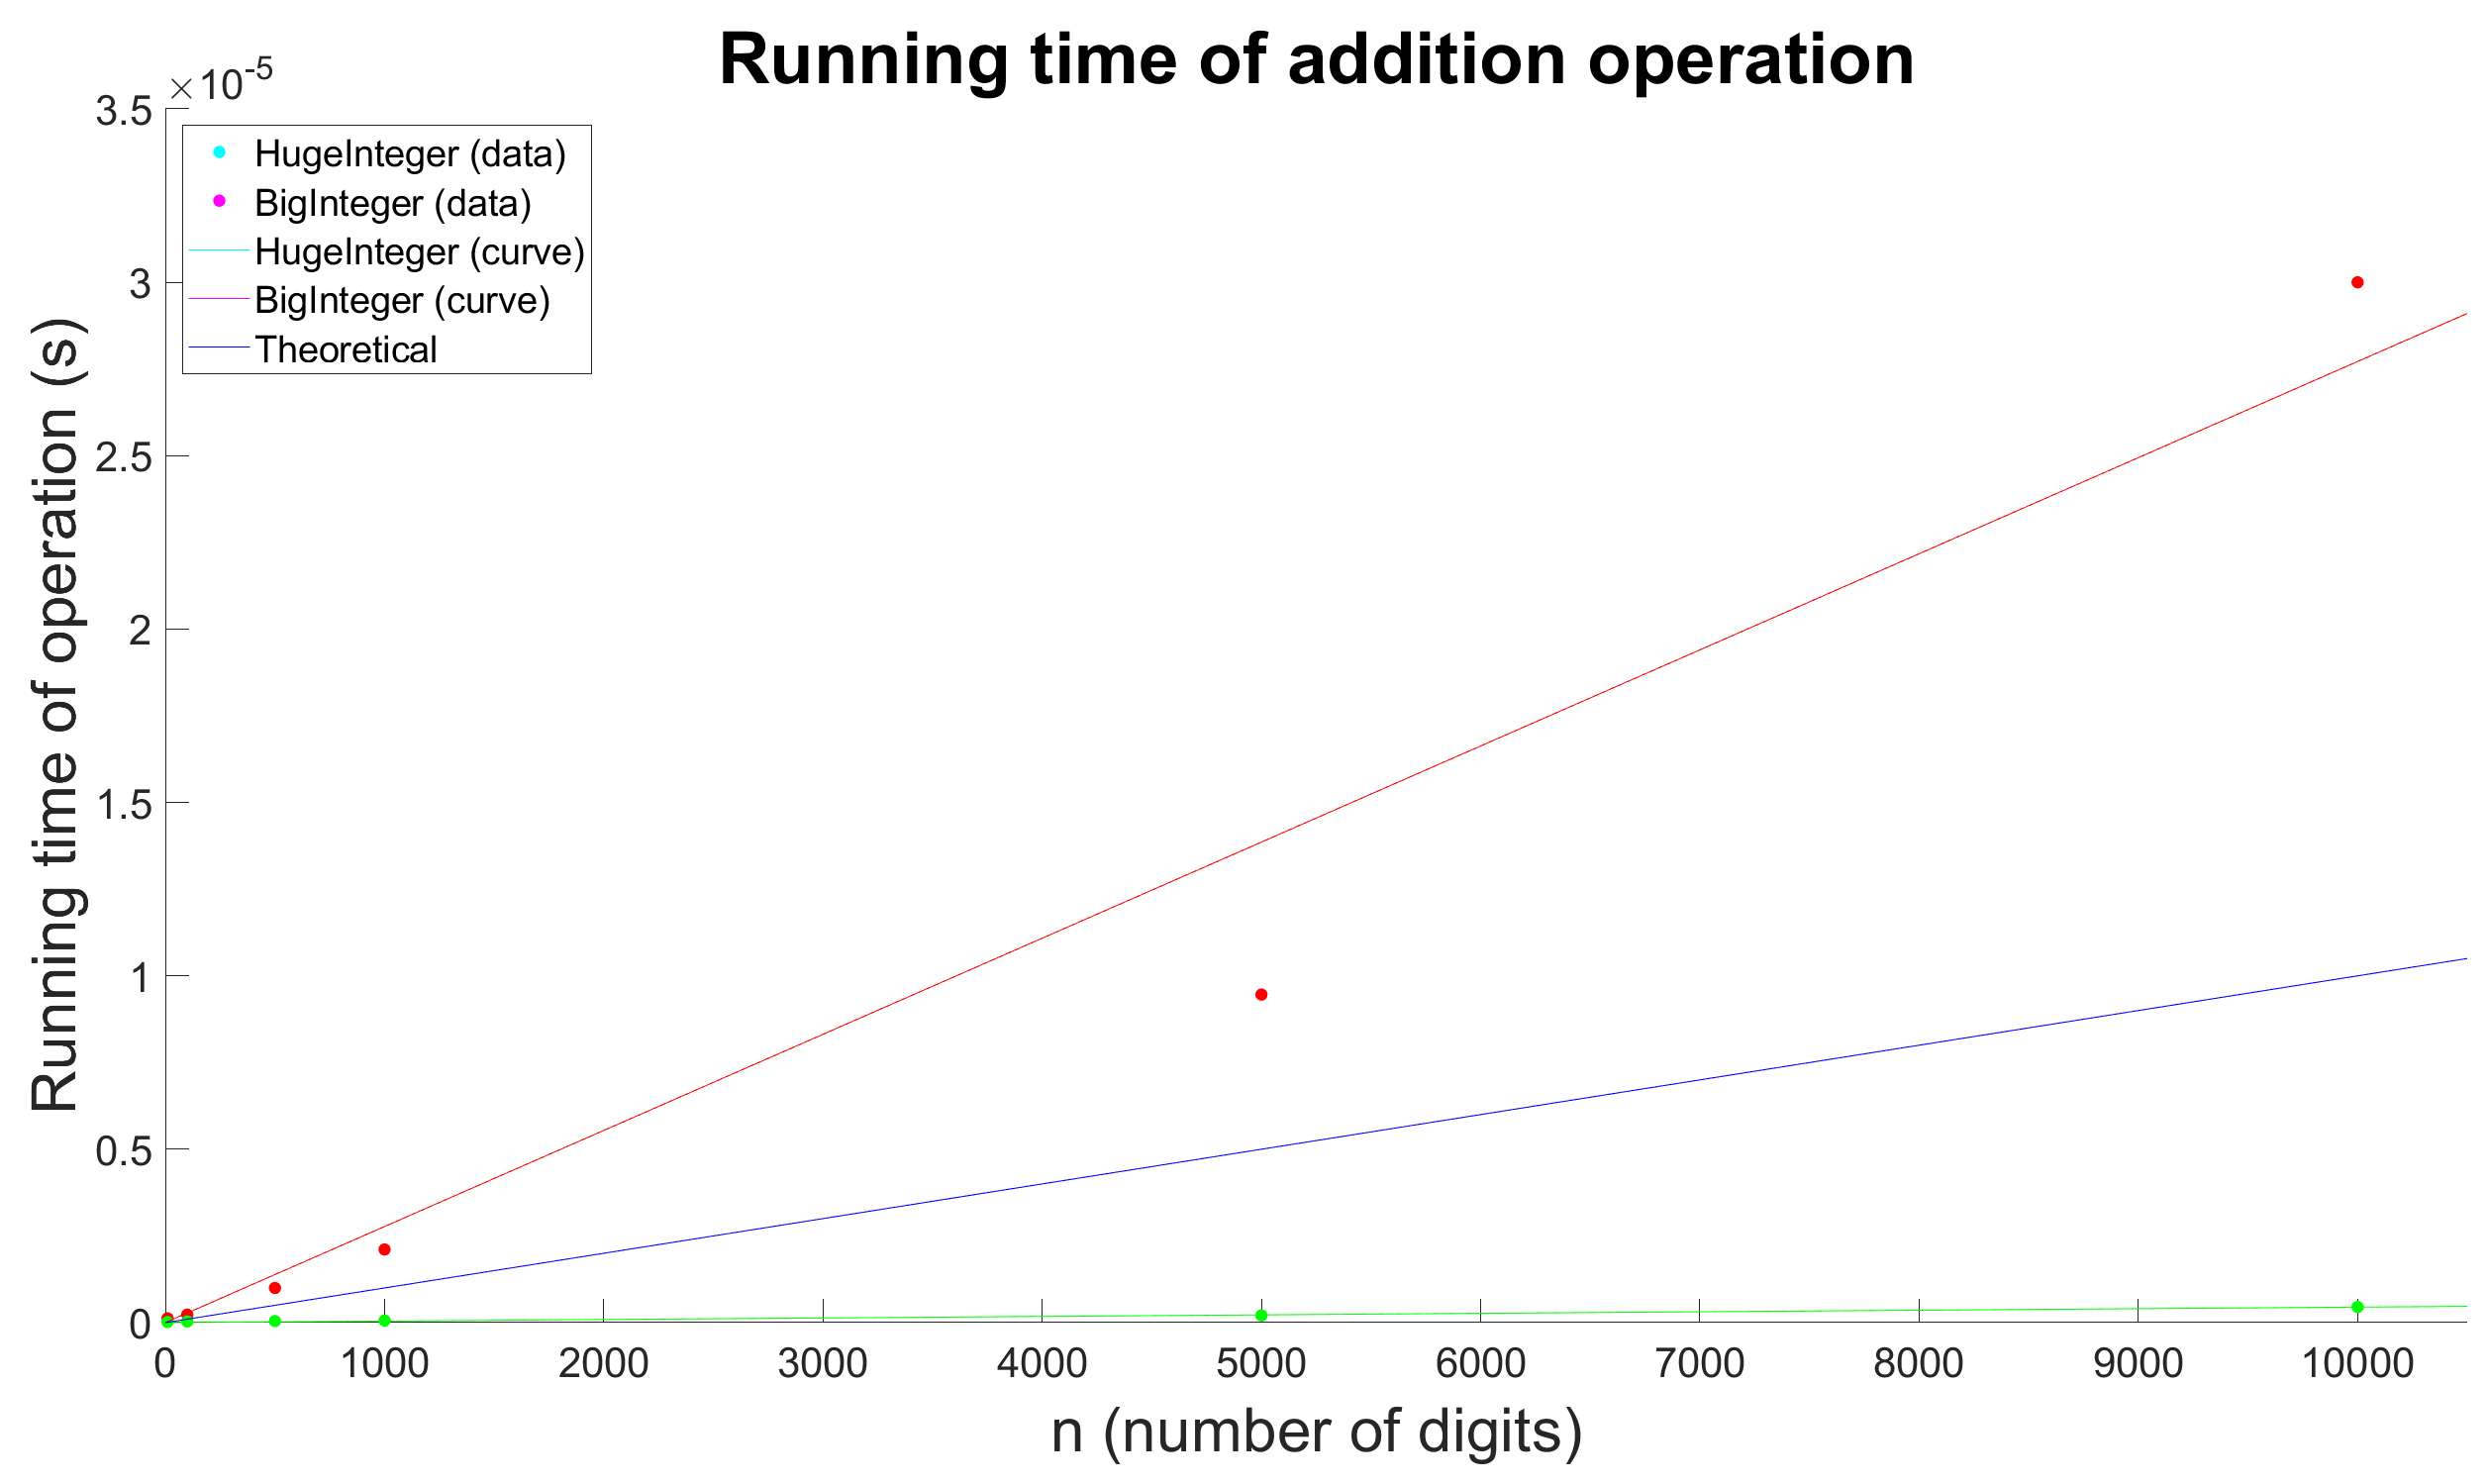
\includegraphics[width=\textwidth]{additionplot.png}
    \caption{Plot of running time for addition operation}
\end{figure}
\begin{figure}[h!]
    \centering
    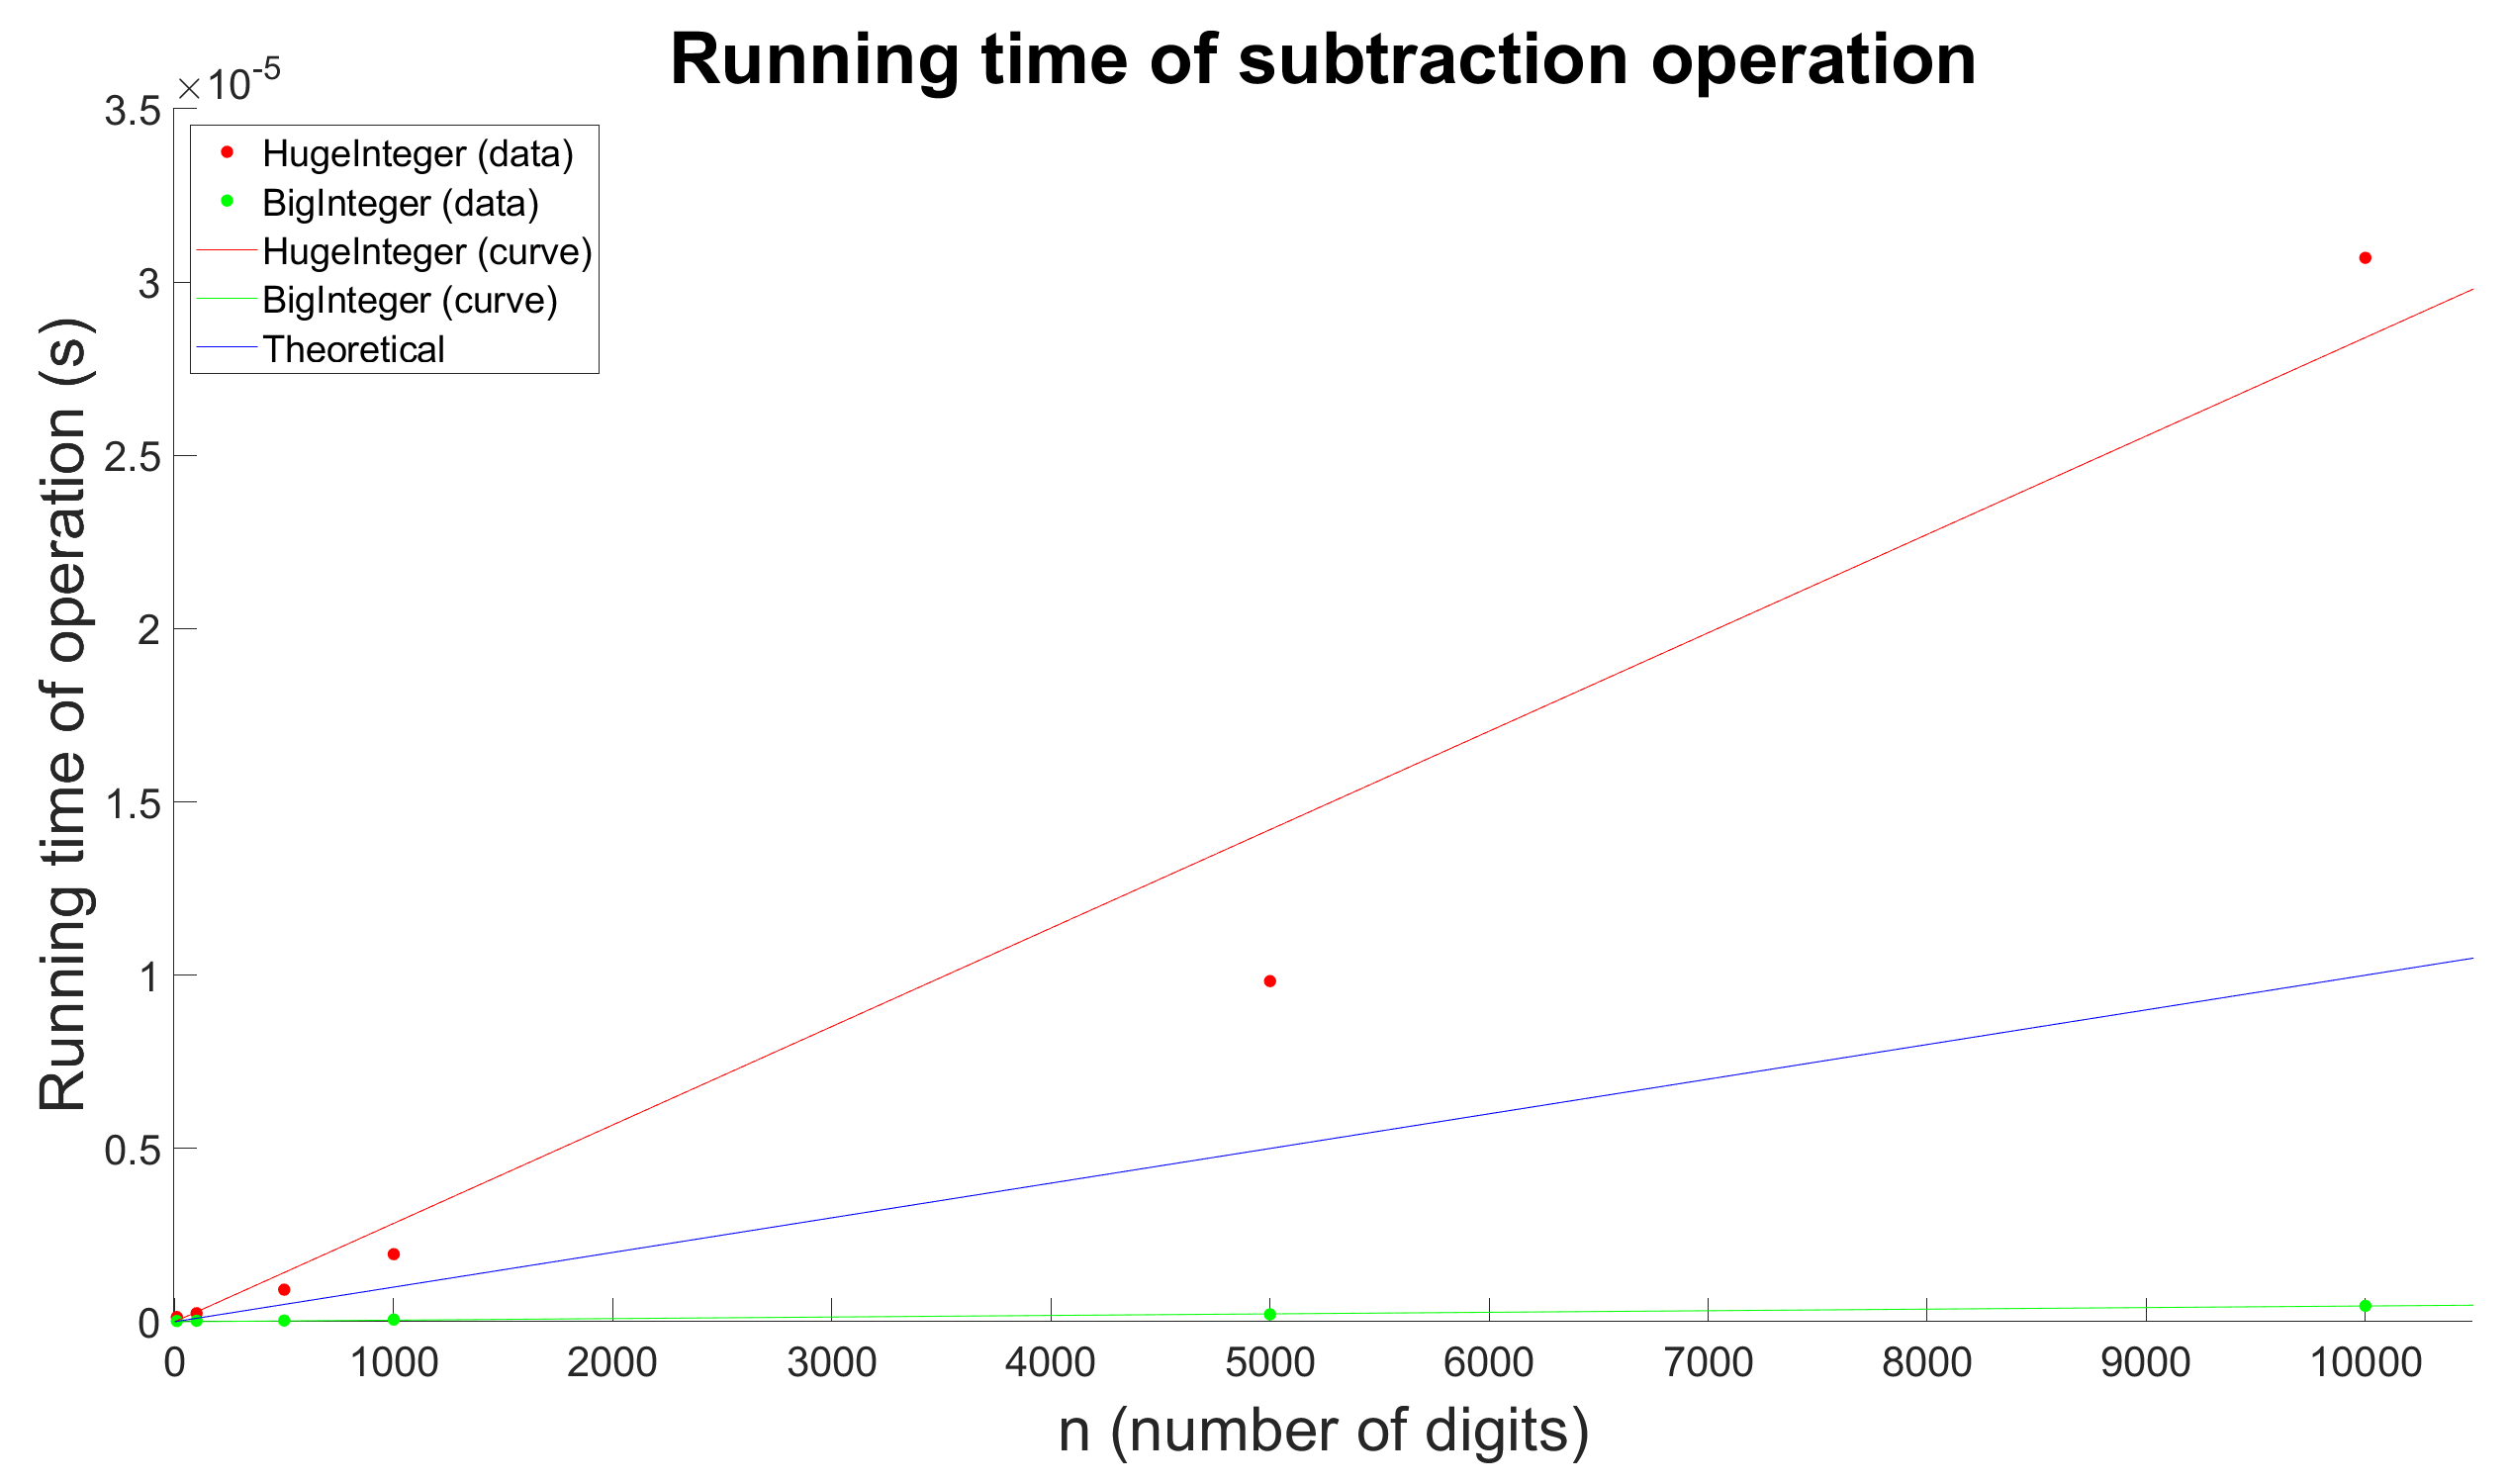
\includegraphics[width=\textwidth]{subtractionplot.png}
    \caption{Plot of running time for subtraction operation}
\end{figure}
\begin{figure}[h!]
    \centering
    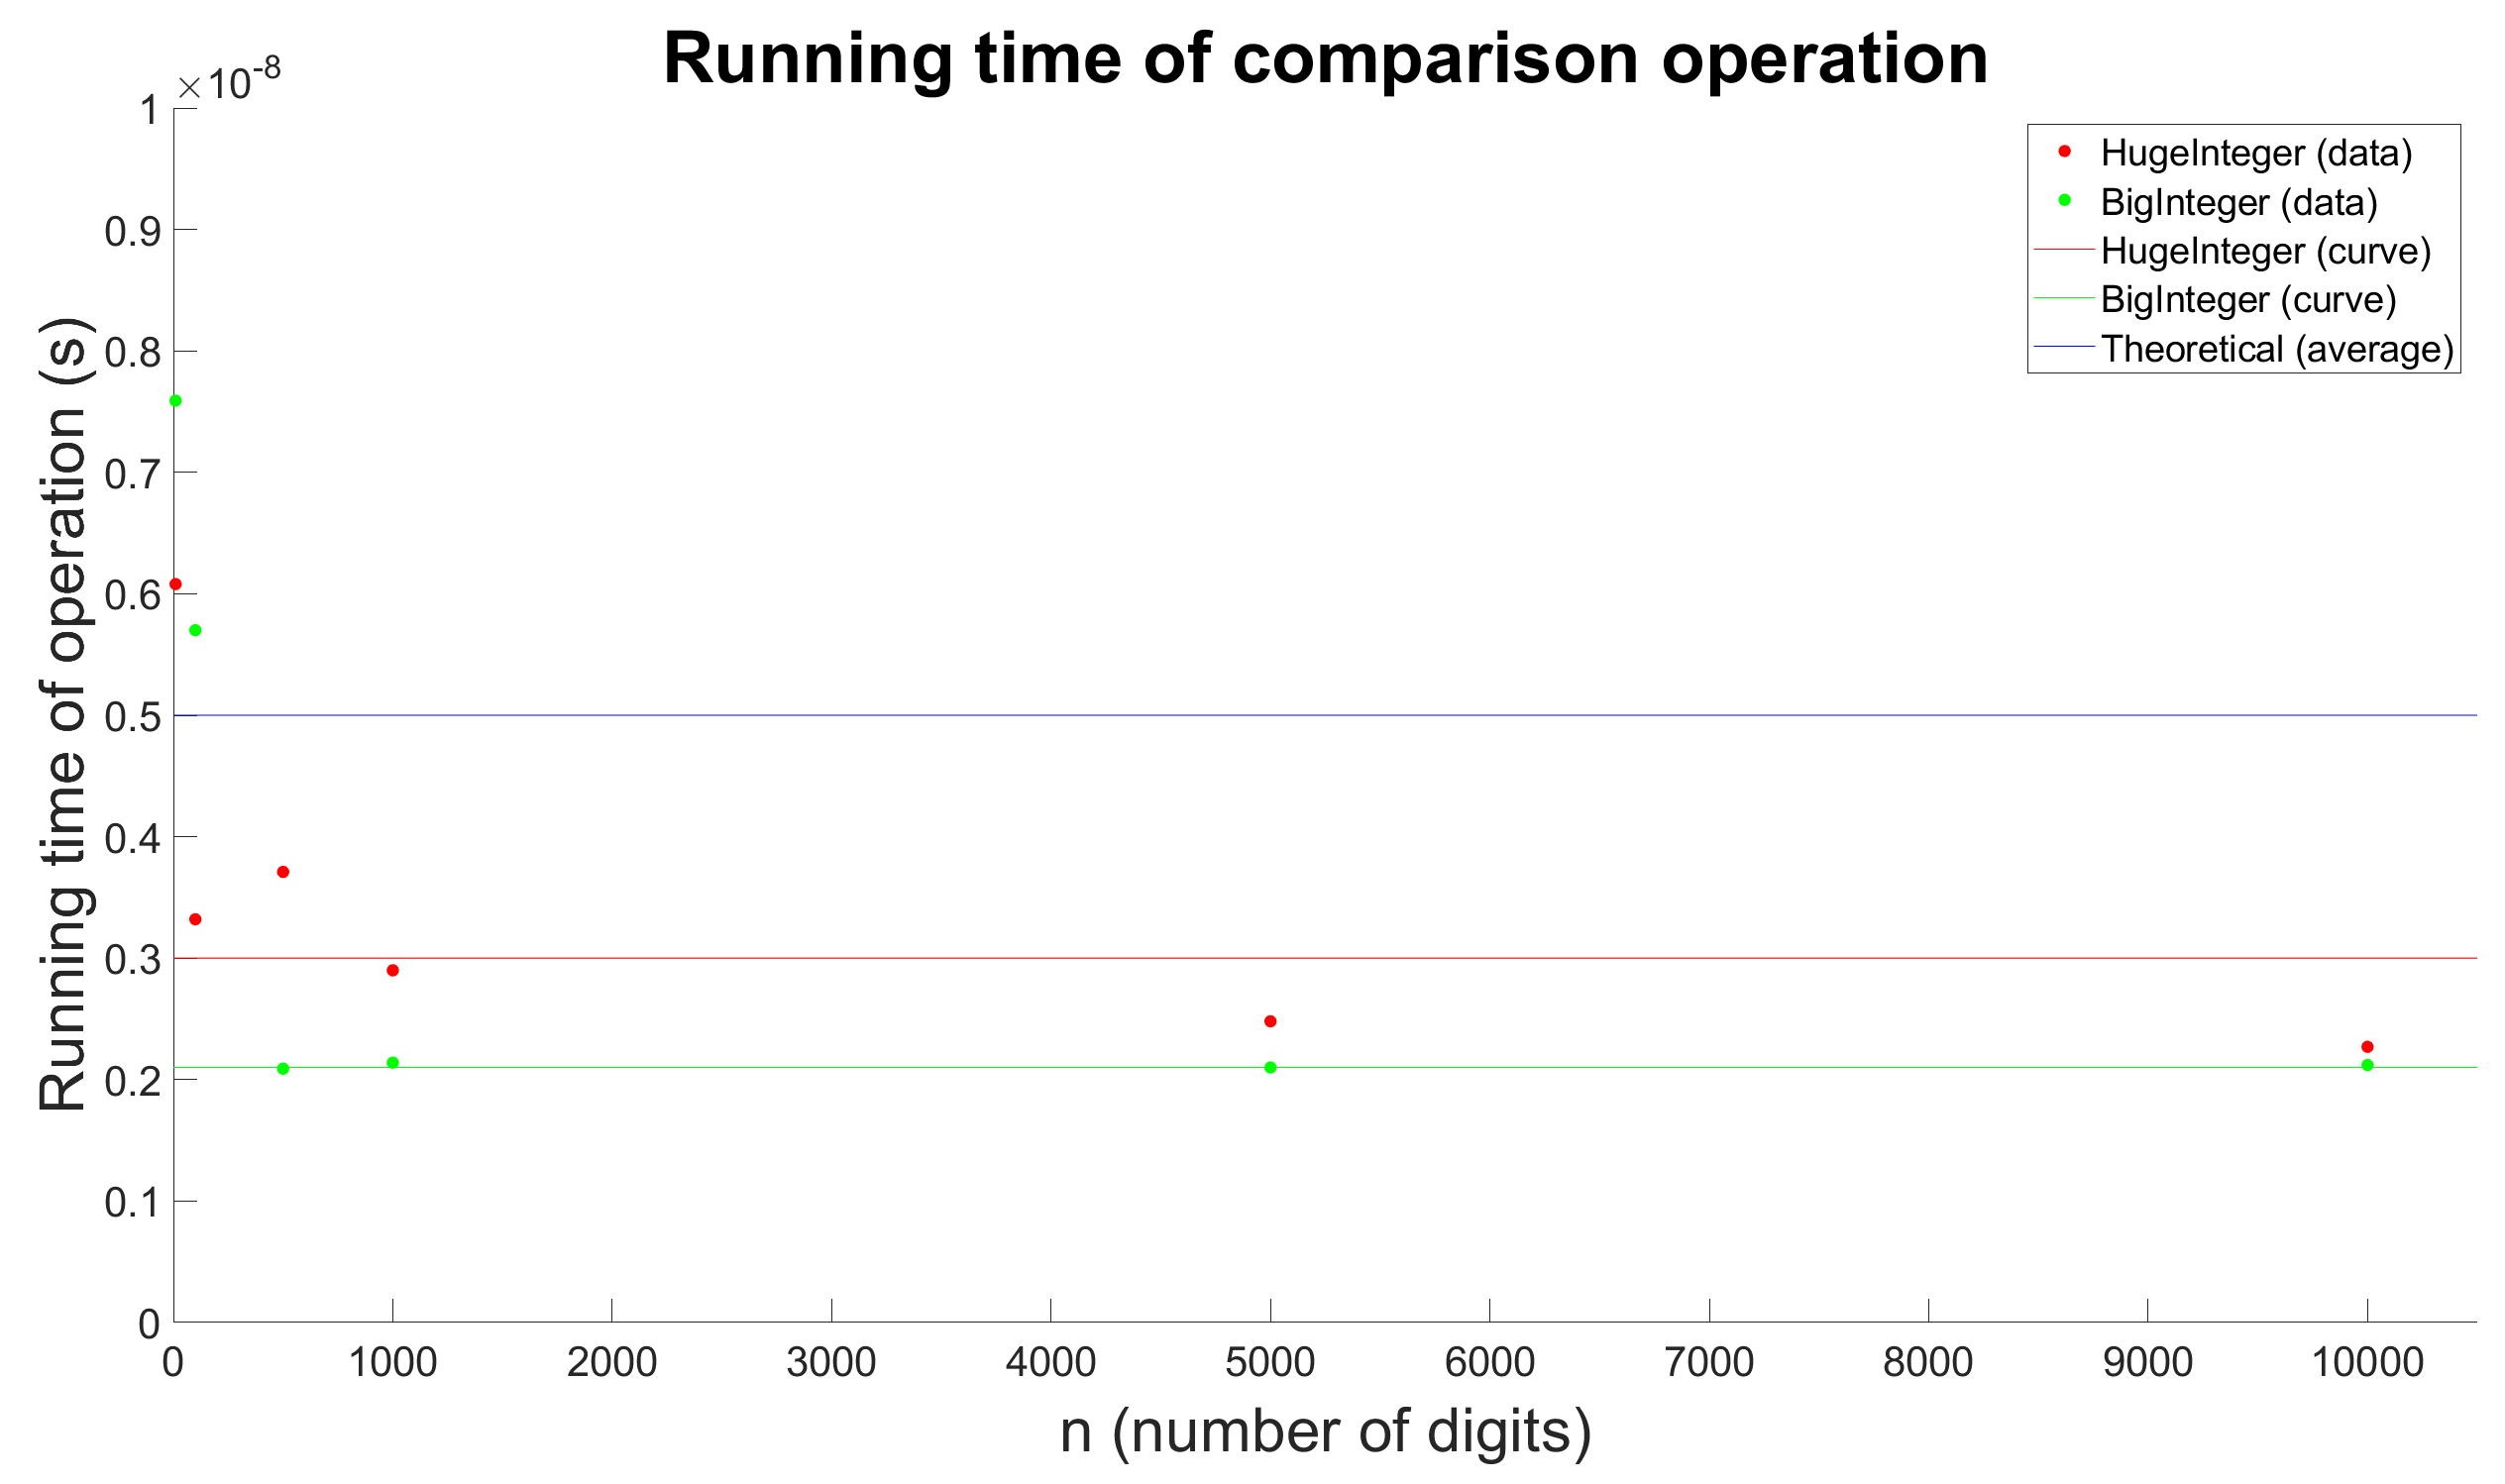
\includegraphics[width=\textwidth]{comparisonplot.png}
    \caption{Plot of running time for comparison operation}
\end{figure}
\begin{figure}[h!]
    \centering
    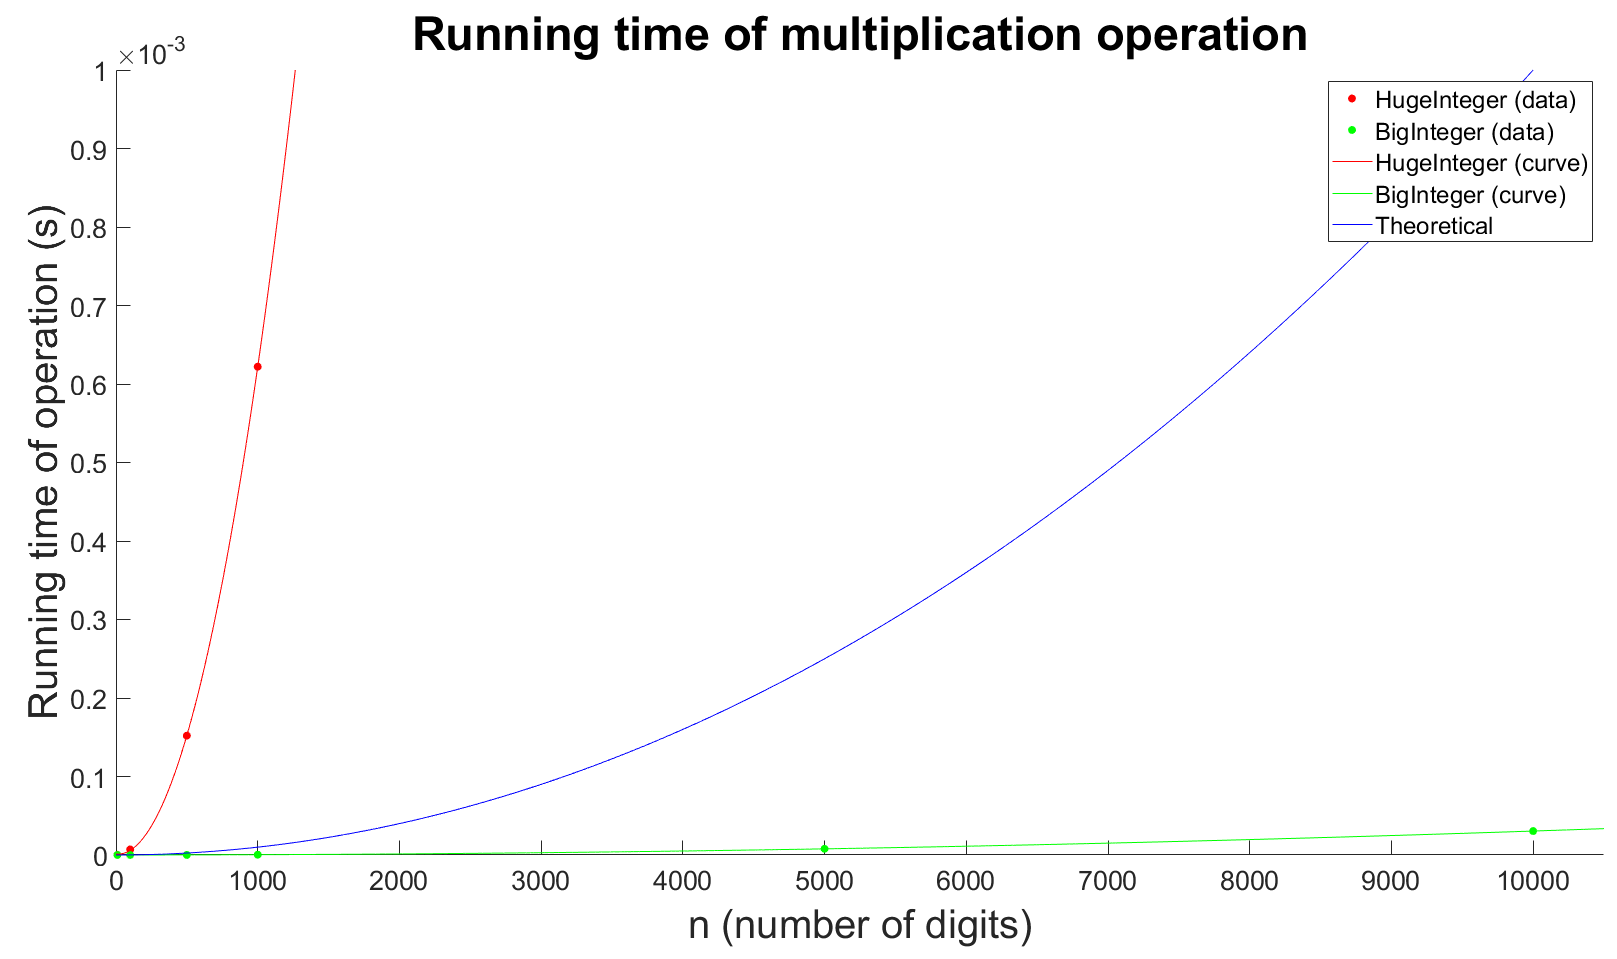
\includegraphics[width=\textwidth]{multiplicationplot.png}
    \caption{Plot of running time for multiplication operation}
\end{figure}

\pagebreak
The only issue with obtaining experimental data occured with the multiplication operation of the \code{HugeInteger} class. The running time at $n=5000$ and $n=10000$ were ommitted because they would take too long to compute at the chosen parameters, and reducing the value of MAXRUNS to speed up the process would introduce too much variance and noise to the data that it would be likely make the data unreliable.

\section*{Discussion of Results and Comparison}
% How well do your theoretical calculations correspond to your measured runningtimes? Do your experimental results make sense? Explain whyor why not.
% How does your implementation compare with thejava.lang.BigIntegerclass interms of running time for each operation?
% Describe any improvements you would make given extra time, which would improvethe running time/memory complexity of your program.
The theoretical calculations correspond relatively well to the measured running times. The experimental results generally follow the same growth rate as the theoretical calculations, and can be modelled relatively acurrately with the growth rate found through calculations. The implementation of \code{HugeInteger} is significantly worse than the implementation \code{java.math.BigInteger}. While the growth rates match relatively well, the actual running times for \code{java.math.BigInteger} is multiple orders of magnitude less in all operations except comparison, which still had a notably smaller running time.

An improvement that could be made to the addition operation that would improve the running time and memory complexity of the both addition and subtraction operations would be to increase the size of the initialized array to equal the maximum possible number of digits and then remove leading zeros at the end, which is how the process is implemented in the multiplication operation. The current implementation removes leading zeros, but also needs to create a new \code{HugeInteger} with an extra digit when the result of the addition requires an extra digit, increasing the memory complexity significantly and also likely increasing the running time as there is an unneeded for loop that the operation must iterate through.

Another potential improvement would be to implement Karatsuba multiplication or an alternative multiplication algorithm that has a lower $\Theta(n)$. A recurvise algorithm like Karatsuba multiplication would increase the memory complexity of the operation, but would significantly increase the running time, as can be seen in the running times for \\ \code{java.math.BigInteger}, which uses Karatsuba multiplication and Toom-Cook multiplication for multiplication of large integers.

\section*{Discussions with Peers and Sources of Inspiration}
\begin{itemize}
    \item The implementation of \code{java.math.BigInteger} in \code{Java 13.0.1}
\end{itemize}
\end{document}